\documentclass[tikz,border=15pt]{standalone}
\usepackage{tikz}
\usepackage{xcolor}
\usetikzlibrary{arrows.meta,calc,positioning,shapes.geometric}

\definecolor{bgcolor}{RGB}{15,23,42}
\definecolor{cardbg}{RGB}{30,41,59}
\definecolor{cardborder}{RGB}{51,65,85}
\definecolor{mhabg}{RGB}{234,88,12}
\definecolor{mhaborder}{RGB}{249,115,22}
\definecolor{ffnbg}{RGB}{2,132,199}
\definecolor{ffnborder}{RGB}{56,189,248}
\definecolor{normbg}{RGB}{234,179,8}
\definecolor{normborder}{RGB}{250,204,21}
\definecolor{embbg}{RGB}{147,51,234}
\definecolor{embborder}{RGB}{192,132,252}
\definecolor{smaxbg}{RGB}{22,163,74}
\definecolor{smaxborder}{RGB}{74,222,128}
\definecolor{encborder}{RGB}{56,189,248}
\definecolor{decborder}{RGB}{236,72,153}
\definecolor{residcolor}{RGB}{251,191,36}
\definecolor{slategray}{RGB}{148,163,184}

\begin{document}
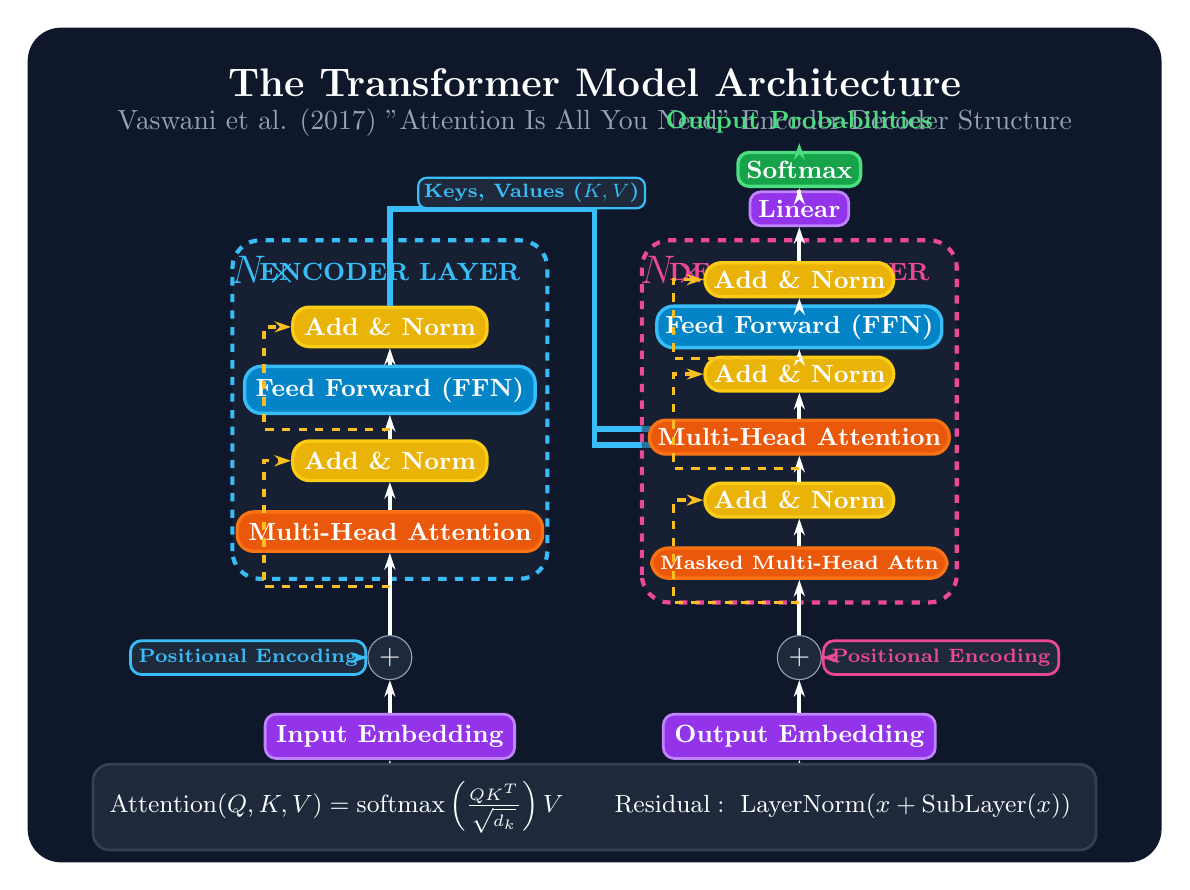
\begin{tikzpicture}[
    >={Stealth[length=6pt, width=4pt]}
]

% Background Card
\fill[rounded corners=12pt, fill=bgcolor] (-7.2,-5.4) rectangle (7.2,5.2);

% Title & Header
\node[text=white, font=\Large\bfseries] at (0, 4.5) {The Transformer Model Architecture};
\node[text=slategray, font=\normalsize] at (0, 4.0) {Vaswani et al. (2017) "Attention Is All You Need" Encoder-Decoder Structure};

% Column Coordinates: Encoder at x = -2.5, Decoder at x = 2.5
\def\ex{-2.6}
\def\dx{2.6}

% 1. ENCODER COLUMN
% Outer Stack Bounding Box (Nx)
\draw[encborder, dashed, line width=1.5pt, fill=cardbg, fill opacity=0.5, rounded corners=10pt] (\ex-2.0, -1.8) rectangle (\ex+2.0, 2.5);
\node[text=encborder, font=\Large\bfseries] at (\ex-1.6, 2.1) {$N\times$};
\node[text=encborder, font=\small\bfseries] at (\ex, 2.1) {ENCODER LAYER};

% Inputs & Embedding
\node[text=white, font=\small\bfseries] (IN_TOK) at (\ex, -4.5) {Inputs};
\node[fill=embbg, draw=embborder, line width=1pt, rounded corners=4pt, text=white, font=\small\bfseries, inner sep=4pt] (IN_EMB) at (\ex, -3.8) {Input Embedding};
\draw[white, line width=1.5pt, ->] (IN_TOK) -- (IN_EMB);

% Sum & Positional Encoding
\node[draw=slategray, fill=cardbg, circle, inner sep=2pt, text=white, font=\bfseries] (IN_SUM) at (\ex, -2.8) {$+$};
\draw[white, line width=1.5pt, ->] (IN_EMB) -- (IN_SUM);

\node[fill=cardbg, draw=encborder, line width=1pt, rounded corners=4pt, text=encborder, font=\scriptsize\bfseries, inner sep=3pt] (IN_POS) at (\ex-1.8, -2.8) {Positional Encoding};
\draw[encborder, line width=1.2pt, ->] (IN_POS) -- (IN_SUM);

% Encoder Sublayers
\node[fill=mhabg, draw=mhaborder, line width=1.2pt, rounded corners=6pt, text=white, font=\small\bfseries, inner sep=4pt] (ENC_MHA) at (\ex, -1.2) {Multi-Head Attention};
\draw[white, line width=1.5pt, ->] (IN_SUM) -- (ENC_MHA);

\node[fill=normbg, draw=normborder, line width=1.2pt, rounded corners=6pt, text=white, font=\small\bfseries, inner sep=4pt] (ENC_NORM1) at (\ex, -0.3) {Add \& Norm};
\draw[white, line width=1.5pt, ->] (ENC_MHA) -- (ENC_NORM1);
% Residual 1
\draw[residcolor, dashed, line width=1.2pt, ->] (\ex, -1.9) -- (\ex-1.6, -1.9) -- (\ex-1.6, -0.3) -- (ENC_NORM1.west);

\node[fill=ffnbg, draw=ffnborder, line width=1.2pt, rounded corners=6pt, text=white, font=\small\bfseries, inner sep=4pt] (ENC_FFN) at (\ex, 0.6) {Feed Forward (FFN)};
\draw[white, line width=1.5pt, ->] (ENC_NORM1) -- (ENC_FFN);

\node[fill=normbg, draw=normborder, line width=1.2pt, rounded corners=6pt, text=white, font=\small\bfseries, inner sep=4pt] (ENC_NORM2) at (\ex, 1.4) {Add \& Norm};
\draw[white, line width=1.5pt, ->] (ENC_FFN) -- (ENC_NORM2);
% Residual 2
\draw[residcolor, dashed, line width=1.2pt, ->] (\ex, 0.1) -- (\ex-1.6, 0.1) -- (\ex-1.6, 1.4) -- (ENC_NORM2.west);

% Cross-Attention Connection to Decoder
\draw[encborder, line width=2pt, ->] (ENC_NORM2.north) -- (\ex, 2.9) -- (0.0, 2.9) -- (0.0, 0.1) -- (\dx-1.4, 0.1);
\draw[encborder, line width=2pt, ->] (0.0, 0.1) -- (0.0, -0.1) -- (\dx-1.4, -0.1);
\node[fill=cardbg, draw=encborder, line width=0.8pt, rounded corners=3pt, text=encborder, font=\scriptsize\bfseries, inner sep=2pt] at (-0.8, 3.1) {Keys, Values ($K, V$)};

% 2. DECODER COLUMN
% Outer Stack Bounding Box (Nx)
\draw[decborder, dashed, line width=1.5pt, fill=cardbg, fill opacity=0.5, rounded corners=10pt] (\dx-2.0, -2.1) rectangle (\dx+2.0, 2.5);
\node[text=decborder, font=\Large\bfseries] at (\dx-1.6, 2.1) {$N\times$};
\node[text=decborder, font=\small\bfseries] at (\dx, 2.1) {DECODER LAYER};

% Outputs & Embedding
\node[text=white, font=\small\bfseries] (OUT_TOK) at (\dx, -4.5) {Outputs (Shifted Right)};
\node[fill=embbg, draw=embborder, line width=1pt, rounded corners=4pt, text=white, font=\small\bfseries, inner sep=4pt] (OUT_EMB) at (\dx, -3.8) {Output Embedding};
\draw[white, line width=1.5pt, ->] (OUT_TOK) -- (OUT_EMB);

% Sum & Positional Encoding
\node[draw=slategray, fill=cardbg, circle, inner sep=2pt, text=white, font=\bfseries] (OUT_SUM) at (\dx, -2.8) {$+$};
\draw[white, line width=1.5pt, ->] (OUT_EMB) -- (OUT_SUM);

\node[fill=cardbg, draw=decborder, line width=1pt, rounded corners=4pt, text=decborder, font=\scriptsize\bfseries, inner sep=3pt] (OUT_POS) at (\dx+1.8, -2.8) {Positional Encoding};
\draw[decborder, line width=1.2pt, ->] (OUT_POS) -- (OUT_SUM);

% Decoder Sublayers
\node[fill=mhabg, draw=mhaborder, line width=1.2pt, rounded corners=6pt, text=white, font=\scriptsize\bfseries, inner sep=3pt] (DEC_MASK) at (\dx, -1.6) {Masked Multi-Head Attn};
\draw[white, line width=1.5pt, ->] (OUT_SUM) -- (DEC_MASK);

\node[fill=normbg, draw=normborder, line width=1.2pt, rounded corners=6pt, text=white, font=\small\bfseries, inner sep=3pt] (DEC_NORM1) at (\dx, -0.8) {Add \& Norm};
\draw[white, line width=1.5pt, ->] (DEC_MASK) -- (DEC_NORM1);
% Residual 1
\draw[residcolor, dashed, line width=1.2pt, ->] (\dx, -2.1) -- (\dx-1.6, -2.1) -- (\dx-1.6, -0.8) -- (DEC_NORM1.west);

\node[fill=mhabg, draw=mhaborder, line width=1.2pt, rounded corners=6pt, text=white, font=\small\bfseries, inner sep=3pt] (DEC_CROSS) at (\dx, 0.0) {Multi-Head Attention};
\draw[white, line width=1.5pt, ->] (DEC_NORM1) -- (DEC_CROSS);

\node[fill=normbg, draw=normborder, line width=1.2pt, rounded corners=6pt, text=white, font=\small\bfseries, inner sep=3pt] (DEC_NORM2) at (\dx, 0.8) {Add \& Norm};
\draw[white, line width=1.5pt, ->] (DEC_CROSS) -- (DEC_NORM2);
% Residual 2
\draw[residcolor, dashed, line width=1.2pt, ->] (\dx, -0.4) -- (\dx-1.6, -0.4) -- (\dx-1.6, 0.8) -- (DEC_NORM2.west);

\node[fill=ffnbg, draw=ffnborder, line width=1.2pt, rounded corners=6pt, text=white, font=\small\bfseries, inner sep=3pt] (DEC_FFN) at (\dx, 1.4) {Feed Forward (FFN)};
\draw[white, line width=1.5pt, ->] (DEC_NORM2) -- (DEC_FFN);

\node[fill=normbg, draw=normborder, line width=1.2pt, rounded corners=6pt, text=white, font=\small\bfseries, inner sep=3pt] (DEC_NORM3) at (\dx, 2.0) {Add \& Norm};
\draw[white, line width=1.5pt, ->] (DEC_FFN) -- (DEC_NORM3);
% Residual 3
\draw[residcolor, dashed, line width=1.2pt, ->] (\dx, 1.0) -- (\dx-1.6, 1.0) -- (\dx-1.6, 2.0) -- (DEC_NORM3.west);

% Top Head (Linear, Softmax, Probabilities)
\node[fill=embbg, draw=embborder, line width=1pt, rounded corners=4pt, text=white, font=\small\bfseries, inner sep=3pt] (LIN) at (\dx, 2.9) {Linear};
\draw[white, line width=1.5pt, ->] (DEC_NORM3) -- (LIN);

\node[fill=smaxbg, draw=smaxborder, line width=1.2pt, rounded corners=4pt, text=white, font=\small\bfseries, inner sep=3pt] (SMAX) at (\dx, 3.4) {Softmax};
\draw[white, line width=1.5pt, ->] (LIN) -- (SMAX);

\node[text=smaxborder, font=\small\bfseries] (PROBS) at (\dx, 4.0) {Output Probabilities};
\draw[smaxborder, line width=2pt, ->] (SMAX) -- (PROBS);

% Footer Formula Box
\node[fill=cardbg, draw=cardborder, line width=1pt, rounded corners=6pt, text=white, font=\small, align=center, inner sep=6pt] at (0, -4.7) {
    $\mathrm{Attention}(Q,K,V) = \mathrm{softmax}\left(\frac{QK^T}{\sqrt{d_k}}\right)V \qquad \mathrm{Residual:\ LayerNorm}(x + \mathrm{SubLayer}(x))$
};

\end{tikzpicture}
\end{document}
